% Chinese working paper. Compile with XeLaTeX or Tectonic, not pdfLaTeX.
\documentclass[conference,a4paper]{IEEEtran}
\usepackage{fontspec}
\usepackage{xeCJK}
\IfFontExistsTF{Times New Roman}{\setmainfont{Times New Roman}}{\setmainfont{texgyretermes-regular.otf}[BoldFont=texgyretermes-bold.otf,ItalicFont=texgyretermes-italic.otf,BoldItalicFont=texgyretermes-bolditalic.otf]}
\IfFontExistsTF{SimSun}{\setCJKmainfont{SimSun}[AutoFakeBold=2]}{\setCJKmainfont{FandolSong-Regular}[Extension=.otf,BoldFont=FandolSong-Bold]}
\IfFontExistsTF{SimHei}{\setCJKsansfont{SimHei}}{\setCJKsansfont{FandolHei-Regular}[Extension=.otf]}
\usepackage{amsmath,booktabs,tabularx,array,graphicx,cite}
\usepackage[hidelinks]{hyperref}
\usepackage{url}
\graphicspath{{figures/}}
\setcounter{dbltopnumber}{3}
\renewcommand{\dbltopfraction}{0.95}
\newcolumntype{Y}{>{\raggedright\arraybackslash}X}
\renewcommand{\tablename}{TABLE}
\renewcommand{\figurename}{图}
\renewcommand{\refname}{参考文献}
\renewcommand{\abstractname}{摘要}
\newcommand{\mse}{\mathrm{MSE}}
\newcommand{\mae}{\mathrm{MAE}}
\newcommand{\priceunit}{千美元}
\title{利用房屋照片预测价格：\\从AlexNet改进到预训练特征组合}
\author{\IEEEauthorblockN{Shifeng Chen \qquad Haoxuan Ying}
\IEEEauthorblockA{1686631 \qquad 1255329\\COMP90086 Computer Vision, The University of Melbourne}}
\begin{document}
\maketitle
\raggedbottom

\section{Introduction：任务与解决思路}
本项目使用课程提供的南加州房屋照片预测价格\cite{dataset,spec}。照片能显示建筑外观、庭院和周边环境，但不一定包含位置、面积和内部装修等重要信息。因此，我们关注的不只是最终分数，也包括：模型能从照片中学到什么，哪些改动有帮助，以及哪些问题仍未解决。

我们先用训练集均价和SIFT特征建立比较起点，再训练AlexNet。针对图片尺寸不一和过拟合，比较预处理、训练设置、增强与结构调整。多数改动收益小，简化回归头则在三个种子上都有效。之后转向固定预训练编码器，重点检查“图片内容是否被保留”和“特征相似度是否适合预测价格”。在整图视野、PCA与核带宽对照后，组合三条预测路线，得到验证MSE 52,201.21、MAE 159.58，历史公开榜MSE 47,291.35。本文按发现问题、尝试改进和检查结果的过程展开，而不把所有改动都解释为成功。

\section{Methods：数据与实验设置}
\subsection{数据划分及指标}
仅使用课程的8,000张有标签图像与3,000张测试图像，价格单位为千美元。为减少重复照片影响比较，我们把已发现的完全重复及近重复图片放入同一组，再按组价格分层，固定划分为6,399张训练图和1,601张验证图。两侧没有相同图片编号、已登记的重复组或像素哈希，但仍可能存在未发现的同一房屋照片。所有方法使用这份划分；种子2026、2027、2028只改变训练随机性。测试标签不用于调参，也未添加原始SoCal数据集中的其他图片或房屋信息。

主指标与辅助指标分别为
\begin{equation}
\mse=\frac{1}{n}\sum_{i=1}^{n}(\hat y_i-y_i)^2,\qquad
\mae=\frac{1}{n}\sum_{i=1}^{n}|\hat y_i-y_i|.
\end{equation}
MSE对大误差惩罚更重，MAE表示平均绝对误差，单位分别为$(\text{千美元})^2$和千美元。另检查价格大于1,300的高价房（训练价格的90\%分位数；验证集159张）。随机模型先用种子2026初筛，有希望的方案再用2027、2028复核；三种子均值下降且至少两次配对改善才保留。报告均值和样本标准差，不把它们当作模型集成成绩。

\subsection{建立比较起点}
最简单的方法对所有图片预测训练集均价，用于检查图像是否提供额外信息。传统方法提取灰度SIFT\cite{sift}，构建256词视觉词袋，对词频直方图进行L1、平方根、L2归一化及标准化，接岭回归（$\alpha=10$）。词典、标准化参数和回归器只在训练部分学习。

AlexNet\cite{alexnet}从随机权重训练，由五个卷积层和9216--4096--4096--1回归头组成。价格先除以1,000计算损失，报告时恢复原单位。保留配置为224$\times$224拉伸、通道归一化均值和标准差均为0.5、AdamW学习率与weight decay均为$10^{-4}$、有效批量32（$4\times8$梯度累积）、dropout 0.5。至少训练40轮、最多60轮，早停耐心15轮、改善阈值0.1\%，恢复验证MSE最低的检查点。增强只用于训练，验证关闭增强和Dropout。小头实验将$6\times6$特征投影至128维，加入位置与归一化后对36个token求均值；单层Transformer使用4个注意力头、512维前馈层。

\subsection{预训练特征与模型组合}
先以冻结CLIP ViT-B/32\cite{clip}加标准化岭回归作为迁移学习参照。最终三条路线使用SigLIP~2 So400m NaFlex\cite{siglip2}、PE-Core-L/14和PE-Core-G/14\cite{pe}的图像特征，不更新编码器，也不使用MLLM或现成房价模型。NaFlex保留宽高比，使用576个patch，输出1,152维；PE-L组合官方输入、336像素灰色补边整图和保留宽高各60\%的中心裁剪；PE-G组合官方448像素视图与补边整图。各视图先单位化，拼接后再单位化，得到3,072维PE-L和2,560维PE-G特征。预测部分使用RBF核岭回归（KRR）\cite{krr}：
\begin{equation}
K(x,x')=\exp(-\gamma\|x-x'\|^2),\qquad
\boldsymbol a=(K+\alpha I)^{-1}(\boldsymbol y-\bar y).
\end{equation}
直观上，核衡量图片特征的相似度，$\gamma$控制相似度下降的速度，$\alpha$控制正则化。预测加回训练均价并将负值截为零。普通核搜索$\gamma\in\{1,4,16\}$、$\alpha\in\{0.01,0.1,1,10\}$，NaFlex选择$\gamma=1,\alpha=0.1$。

通用视觉相似并不一定代表价格接近。PE-L因此用PLS\cite{pls}学习价格相关方向：折内拟合16个分量，最终使用前4个标准化得分$s$，核为$\exp(-\|x-x'\|^2-0.1\|s-s'\|^2/4)$，$\alpha=1$。PE-G则用不需要价格的PCA\cite{pca}压缩特征，比较64、256、1,024维及白化幂0、0.5，再单位化。压缩改变距离，因此另比较以下带宽调整：
\begin{equation}
\gamma'=4\frac{\operatorname{median}\|x_i-x_j\|^2}
{\operatorname{median}\|z_i-z_j\|^2},
\end{equation}
其中$z$为变换后特征，中位数用拟合折内固定抽取的8,192对不同图片计算。最终保留不白化的PCA256，$\alpha=1$。PCA、PLS及缩放参数均只在对应训练折学习。

将训练集按组分为三折，每次用两折训练、预测剩下一折，得到每张图片未参与该次训练时的OOF预测。再借鉴堆叠回归\cite{stacking}，用这些预测学习非负且和为1的权重：
\begin{equation}
\hat y=\sum_{j=1}^{3}w_j\hat y_j,\quad
\boldsymbol w=(0.1081,\,0.0808,\,0.8111).
\end{equation}
验证标签不用于拟合权重。用两折OOF预测学权重、在剩下一折评价，记为meta-crossfit；基础模型已被筛选，它不是完全独立测试。新增分支需让meta MSE降低至少1\%、至少两折改善且验证MSE下降。最终固定超参数和权重，在8,000张有标签图上重拟合变换、核带宽与回归器，生成3,000条测试预测。

\section{Results：问题、尝试与改进}
\subsection{先检查图像信息与输入处理}
表\ref{tab:overall}汇总相同验证集上的结果。SIFT相比均价只降低4.28\%的MSE，说明局部图像信息有用，但作用有限。一个可能原因是词袋统计保留了局部纹理，却弱化了它们在图中的位置，难以区分整栋房屋的布局。AlexNet的结果更好，因此我们继续以它为基础检查输入处理和训练方法，而不是只增加传统特征数量。

\begin{table}[t]
\caption{Method overview on the same 1,601 validation images. $\pm$: sample SD across three seeds; other rows: one selected configuration.}
\label{tab:overall}\centering\footnotesize
\setlength{\tabcolsep}{3pt}
\begin{tabularx}{\columnwidth}{Yrr}\toprule
Method & MSE & MAE\\\midrule
Training mean &151,839.69&294.47\\
SIFT--BoVW--Ridge & $145,336.73\!\pm\!1,091.58$ &288.66\\
AlexNet (no aug.) & $127,774.42\!\pm\!486.30$ &264.52\\
AlexNet (H-flip) & $126,810.01\!\pm\!1,902.23$ &268.02\\
Mean-pool head & $122,334.22\!\pm\!1,588.64$ &261.48\\
CLIP B32 + Ridge &91,820.73&223.27\\
NaFlex KRR &63,086.48&181.28\\
PE-L PLS KRR &59,483.31&171.73\\
PCA PE-G KRR &52,805.77&160.67\\
Final fusion &\textbf{52,201.21}&\textbf{159.58}\\\bottomrule
\end{tabularx}
\end{table}

图片大小和比例不一，首先需要统一输入。我们比较等比补边、拉伸、中心裁剪、320分辨率、通道标准化，以及空间/频域低通。频域滤波在种子2026初筛最好（127,610.87），但三种子仅1次胜过对应对照；直接拉伸则2/3改善，均值127,774.42略低于滤波的127,886.38和补边的128,415.68，因此保留拉伸。拉伸可能让房屋占用更多有效像素，但也改变比例；滤波可能减弱无关纹理，也可能丢失有用细节。这些相反作用是收益仅约0.50\%的可能解释，尚不能单独证实。滤波加拉伸也没有超过单项，说明改动不能简单叠加。

我们也检查了学习率、优化器、调度、批量和Dropout。初筛有改善的Adam未在三种子平均结果上胜出，余弦调度也未优于固定学习率。这提示问题可能不只是“没有把训练损失降下来”，因此不再仅围绕优化器寻找提升，而继续检查过拟合和图像信息利用。

\subsection{用增强减少对拍摄条件的依赖}
增强的思路是：同一房屋换一个位置、方向或光照，价格不应改变。如果模型过于依赖这些拍摄条件，训练时加入变化可能有帮助。表\ref{tab:aug}每次只增加一种操作，与无增强AlexNet比较。水平翻转三种子MSE降低0.75\%至126,810.01，2/3种子改善，故保留；但MAE由264.52升至268.02，说明并非所有误差都变小。擦除初筛略好，复核均值却为128,300.21、仅1/3改善，因此放弃。

翻转保留了大部分可见内容，可能比裁剪、擦除更少损失信息。相反，裁剪可能去掉庭院或建筑边缘，模糊和噪声可能遮盖细节；而这些细节本身也可能与价格有关。这可以解释为何增强没有普遍有效，但我们没有逐项验证原因，其他操作也只做了单种子初筛。依据现有结果，我们没有继续叠加未证实有效的增强。

\begin{table}[t]
\caption{Historical augmentation screen (seed 2026). $\Delta$MSE is relative to the same-batch control; negative is better.}
\label{tab:aug}\centering\footnotesize
\setlength{\tabcolsep}{3pt}
\begin{tabularx}{\columnwidth}{Yrr}\toprule
Operation / parameters & MSE & $\Delta$MSE\\\midrule
No augmentation &128,268.67&0\\
H-flip: $p=0.5$ &126,601.97&$-1,666.70$\\
Rotation: $p=0.3$, $\pm3^\circ$ &129,526.18&$+1,257.51$\\
Translation: $p=0.3$, $\pm3\%$/axis &129,162.73&$+894.06$\\
Crop: $p=0.3$, area 90--100\% &130,222.98&$+1,954.31$\\
Blur: $p=0.2$, $\sigma=0.3$--$0.8$ &129,941.36&$+1,672.69$\\
Noise: $p=0.2$, $\sigma=0.01$ &131,174.53&$+2,905.87$\\
Erasing: $p=0.15$, area 1--3\% &128,114.40&$-154.27$\\\bottomrule
\end{tabularx}
\end{table}

后期补做亮度和对比度实验，使用相同初始化、固定划分和种子2026，分别以概率1采样乘数$U(0.9,1.1)$，不叠加其他增强，各训练40轮。表\ref{tab:photo}中亮度MSE基本不变；一种可能是原图已有照明差异，小幅亮度变化没有补充多少新变化。对比度MSE下降1.93\%，可能减轻了对特定明暗纹理的依赖，但高价房MSE反而增加17.14\%。我们无法确定这是细节被削弱还是训练波动，因此只将其列为待复核方案，没有加进最终模型。这组结果只与同期控制组131,389.94比较，不与旧批次混比。

\begin{table}[t]
\caption{Photometric screen with a fresh, same-batch control (one seed). Tail: 159 images with price $>1,300$ thousand USD.}
\label{tab:photo}\centering\footnotesize
\setlength{\tabcolsep}{3pt}
\begin{tabularx}{\columnwidth}{Yrrr}\toprule
Setting & MSE & MAE & Tail MSE\\\midrule
Control &131,389.94&282.64&593,970.49\\
Brightness &131,433.91&274.50&616,903.93\\
Contrast &128,860.53&269.01&695,747.66\\\bottomrule
\end{tabularx}
\end{table}

\subsection{训练表现停滞时，是否应增加复杂度？}
光度对照的最佳验证点在第7、11和5轮，此后训练误差下降却未持续改善验证表现，与过拟合相符。因此使用最佳检查点而非最后一轮；训练开启Dropout及对应增强，不能把训练、验证曲线间距直接视为同条件误差差距。
为改善特征提取，我们在翻转AlexNet上分别尝试小卷积核堆叠、多尺度块和残差块。同种子对照为126,601.97，三种改动分别为127,319.95、130,027.49和128,714.26，均未保留。这些只是AlexNet上的局部改动，不是完整VGG、Inception和ResNet比较。可能的原因是增加结构没有解决训练样本和价格线索有限的问题，还增加了学习难度；初筛结果不足以证明这些结构普遍无效。

随后改用平均池化小回归头，三种子MSE降至122,334.22，三次均优于翻转AlexNet。较小的头减少需要拟合的参数，平均池化也降低了对具体空间位置的依赖，这可能使其更不容易记住训练图片，但两种作用尚未拆开验证。再加单层Transformer后，种子2026的MSE从小头的120,774.16变为124,389.28。因此我们保留简单的小头，没有继续加深。结果提示：对当前数据，更复杂不一定更合适。

接下来固定预训练特征，只学习房价预测部分。CLIP加岭回归的MSE降至91,820.73，较小头改善约24.94\%，这使我们进一步探索SigLIP2和PE。可能是预训练特征已包含较丰富的形状、纹理和场景信息，不必仅靠6,399张图从头学习。但编码器和回归器同时改变，这不是单独证明预训练效果的消融。

\subsection{补充视野后，为什么PCA一度变差？}
预训练模型也可能在输入裁剪时丢失内容。为此保留PE-G官方视图，再补充整图，而不是用整图完全替换。验证MSE由55,097.49降至53,252.81，OOF MSE由55,679.73降至53,646.46，支持补充视野有用。可能是边缘房屋或周边环境得到保留，但这不能证明所有背景都有帮助。

随后尝试压缩特征，PCA256沿用$\gamma=4$时，OOF MSE反而升至77,771.43。我们没有直接判定PCA无效，而检查它是否同时改变了核计算。图\ref{fig:pca}显示，变换并单位化后，训练图片对的平方距离中位数从0.5402升至2.0515；相同$\gamma$下，RBF相似度因此明显减小。按式(3)调整带宽后，开发训练拟合的$\gamma'$为1.05323，OOF MSE降至52,531.27，验证MSE为52,805.77。这说明“换特征但保持原参数”不一定是公平比较，需要检查下游算法是否仍适用。距离图支持尺度变化这一解释，但未证明PCA只移除了无关信息。

加入该分支后，原组合meta MSE从53,052.57降至52,210.22，三折均改善；验证MSE从52,524.78降至52,201.21，达到保留条件。历史公榜相应由47,837.69降至47,291.35，但该分数不替代训练侧和验证集比较。
\begin{figure*}[t]
\centering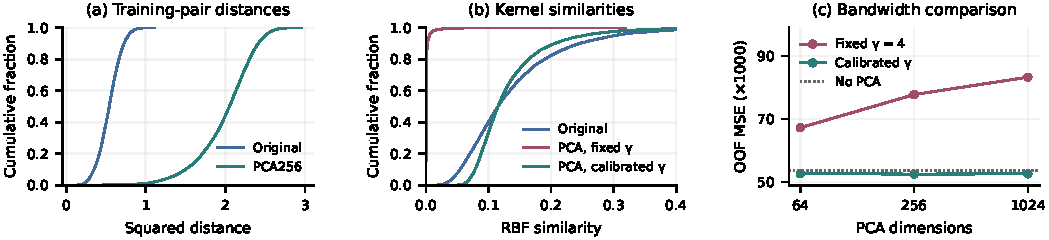
\includegraphics[width=\textwidth]{report_pca_distance_bandwidth_oof.pdf}
\caption{PE-G的PCA诊断。(a) 8,192对训练图片的平方距离分布；(b) RBF相似度分布（显示0--0.4）；(c) 不白化PCA在固定与校准带宽下的三折OOF MSE。所有变换和带宽只用拟合折计算。}
\label{fig:pca}
\end{figure*}

\subsection{组合是否真的比单个模型好？}
不同特征可能在不同图片上出错，因此我们进一步尝试加权平均预测，而不是只选一个模型。表\ref{tab:ablation}逐次移除一条路线，只在训练OOF上重学剩余权重。PCA PE-G单独为52,805.77，完整组合为52,201.21，仅再改善约1.14\%。移除PE-G后升至57,372.90，而移除NaFlex升至52,597.50，说明主要提升来自强单模型，其他模型只提供小幅补充。可能是它们的错误部分重合，组合无法纠正大家都预测不准的图片；尚需逐图误差相关分析验证。等权组合反而较差（53,847.68），也说明不应让较弱模型占同等比重。

\begin{table}[t]
\caption{Fusion ablation. Validation: $n=1,601$; meta: three-fold cross-fitting on 6,399 training-side OOF predictions, not an independent test.}
\label{tab:ablation}\centering\footnotesize
\setlength{\tabcolsep}{3pt}
\begin{tabularx}{\columnwidth}{Yrr}\toprule
Configuration & Val. MSE & Meta MSE\\\midrule
NaFlex only &63,086.48&64,475.13\\
PE-L PLS only &59,483.31&59,515.43\\
PCA PE-G only &52,805.77&52,531.27\\
No NaFlex; refit weights &52,597.50&52,359.30\\
No PE-L PLS; refit weights &52,194.81&52,244.24\\
No PCA PE-G; refit weights &57,372.90&57,694.20\\
Equal-weight fusion &53,847.68&54,214.33\\
Frozen full fusion &52,201.21&52,210.22\\\bottomrule
\end{tabularx}
\end{table}

PE-L PLS是否值得保留还不明确：去掉它后验证MSE低6.40（约0.012\%），但meta MSE高34.02，方向不一致，不能据此认定删除更好。后续尝试校正预测的整体偏移与尺度，以及用无约束岭回归组合预测，meta MSE分别为52,251.89和52,256.36，也未超过原方案52,210.22。因此保持最终方案不变。这里移除的是整条预测路线，不能当作单独验证PCA或PLS的实验，也未对小幅差异做显著性检验。

\subsection{平均分数之外：哪些图片仍然困难？}
最终RMSE为228.48、绝对误差中位数113.41，平均偏差只有$+6.51$，但图\ref{fig:errors}显示低价高估和高价低估相互抵消。最低价组MAE为104.03，高价组为410.90、平均低估385.16。高价组仅占9.93\%样本，却贡献47.13\%平方误差；误差最大的161张贡献63.30\%。最后一步组合改善也不均匀：最低、最高价位对总MSE变化分别贡献$-224.23$、$-882.25$，中间两组则为$+185.43$、$+597.48$。总变化$-323.57$并不代表每组都改善。

图\ref{fig:occlusion}进一步检查补充视野何时有用。我们在1,543张横向验证图中选择改善最大4920与退步最大5712，而非随机选例。4920真实874.5，单视图预测约1,370，双视图降至1,192，更接近真实值；5712真实1,250，却由1,274升至1,496。补充场景有时纠正估计，有时反而带来误导，因此不能把“看得更多”直接等同“预测更准”。

参考区域遮挡方法\cite{occlusion}，将图片分成$4\times4$格，分别用灰色或半径8的高斯模糊内容替换一格，记录预测变化。图中较强响应与房屋区域重叠，但5712双视图模型的灰色/模糊响应相关系数仅0.267，说明解释依赖替换方式。这些图只反映三种PE-G回归流程对扰动的敏感性，不是分割、因果证据或最终三模型组合的解释图。
\begin{figure*}[t]
\centering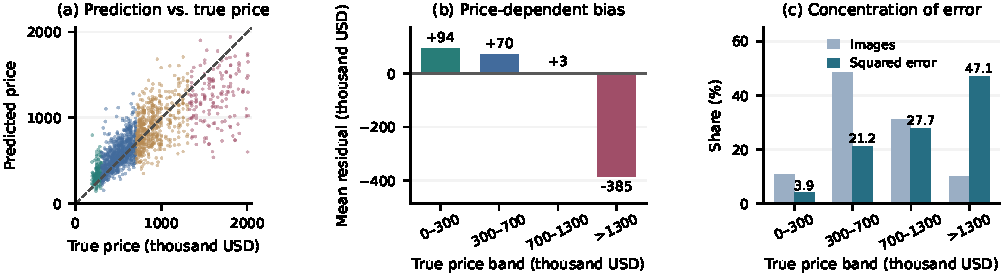
\includegraphics[width=\textwidth]{report_prediction_scatter_price_band_errors.pdf}
\caption{最终组合在1,601张验证图上的误差。(a) 预测与真实价格；(b) 各价位平均误差（预测减真实）；(c) 样本与平方误差占比。四组为$(0,300]$、$(300,700]$、$(700,1300]$、$>1300$千美元，数量依次169、775、498、159。}
\label{fig:errors}
\end{figure*}
\begin{figure*}[t]
\centering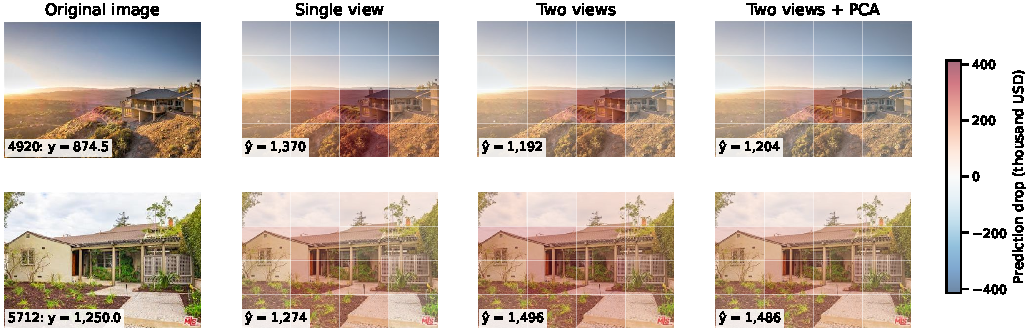
\includegraphics[width=\textwidth]{report_pe_g_occlusion_model_comparison.pdf}
\caption{PE-G区域模糊替换对照：单视图、双视图、双视图加PCA。红色表示替换后预测下降，蓝色表示上升；统一色标单位为千美元。两例分别是加入整图后改善最大和退步最大的横向验证图片，不代表总体表现。}
\label{fig:occlusion}
\end{figure*}

\section{Discussion：经验、局限与下一步}
这次实验使我们逐步认识到，提升不只来自增加模型复杂度。SIFT保留局部纹理，却弱化布局；从零训练CNN能学习布局，但需要同时学习特征和价格关系，较小的回归头反而更稳定。冻结编码器提供了已有视觉知识，使我们能集中改进视野和回归方式。不过，PCA失败再恢复的例子说明，即使特征更紧凑，下游相似度计算也必须配套调整，不能只看操作本身是否常用。

高价低估可能与高价样本较少、外观信息不充分有关，但当前实验不能分离这些原因。单张照片无法直接告诉我们位置、面积或交易条件；遮挡图也不能证明模型真正理解了某个定价因素。后续应先检查高误差图片中的遮挡、主体大小与场景差异，再设计内容覆盖的对照。可尝试提高高价样本抽样比例，但必须同时检查普通价位，避免转移误差；对比度应先多种子复核并测试更小幅度。这些是尚未验证的计划，不需要增加课程以外的房屋数据。

反复使用同一验证集会带来选择偏差，meta-crossfit也未消除先前筛选模型的影响；小幅差异应在预先固定的额外分组评价中复核。通用预训练数据来源不能完全核验，我们未添加额外SoCal数据，但不保证预训练零重叠。缓存特征减少重复计算，不代表大型编码器和稠密核没有成本。公开榜、固定验证及meta分数来自不同数据与流程，不能相互替代。最终保留三模型组合，主要依赖PE-G，承认其他分支收益有限及高价误差仍大；更重要的收获是用对照结果决定下一步，而不是将所有尝试都累加进最终模型。

% Flush every result figure within the four-page body; references may use page five.
\clearpage
\begin{thebibliography}{12}
\bibitem{dataset} T. Dogan, ``House Prices and Images -- SoCal,'' 2019. [Online]. Available: \url{https://www.kaggle.com/datasets/ted8080/house-prices-and-images-socal}. 数据来源引用；实验仅使用课程提供子集。
\bibitem{spec} The University of Melbourne, ``COMP90086 Computer Vision: Predicting House Prices,'' Semester 2, 2026, project specification.
\bibitem{sift} D. G. Lowe, ``Distinctive Image Features from Scale-Invariant Keypoints,'' \emph{International Journal of Computer Vision}, vol.60, no.2, pp.91--110, 2004.
\bibitem{alexnet} A. Krizhevsky, I. Sutskever, and G. E. Hinton, ``ImageNet Classification with Deep Convolutional Neural Networks,'' in \emph{Advances in Neural Information Processing Systems}, vol.25, 2012.
\bibitem{clip} A. Radford et al., ``\href{https://proceedings.mlr.press/v139/radford21a.html}{Learning Transferable Visual Models From Natural Language Supervision},'' in \emph{Proc. ICML}, 2021, pp.8748--8763.
\bibitem{siglip2} M. Tschannen et al., ``SigLIP 2: Multilingual Vision-Language Encoders with Improved Semantic Understanding, Localization, and Dense Features,'' arXiv:2502.14786, 2025.
\bibitem{pe} D. Bolya et al., ``Perception Encoder: The best visual embeddings are not at the output of the network,'' arXiv:2504.13181, 2025.
\bibitem{krr} C. Saunders, A. Gammerman, and V. Vovk, ``Ridge regression learning algorithm in dual variables,'' in \emph{Proc. ICML}, 1998, pp.515--521.
\bibitem{pls} S. Wold, A. Ruhe, H. Wold, and W. J. Dunn III, ``The collinearity problem in linear regression. The partial least squares (PLS) approach to generalized inverses,'' \emph{SIAM J. Sci. Stat. Comput.}, vol.5, pp.735--743, 1984.
\bibitem{pca} K. Pearson, ``On lines and planes of closest fit to systems of points in space,'' \emph{Philosophical Magazine}, vol.2, pp.559--572, 1901.
\bibitem{stacking} L. Breiman, ``Stacked regressions,'' \emph{Machine Learning}, vol.24, pp.49--64, 1996.
\bibitem{occlusion} M. D. Zeiler and R. Fergus, ``\href{https://arxiv.org/abs/1311.2901}{Visualizing and Understanding Convolutional Networks},'' in \emph{Proc. ECCV}, 2014, pp.818--833.
\end{thebibliography}
\end{document}
